\documentclass{standalone}
% Preamble
\begin{document}

\subsection{Structure bloc-triangulaire et rang numérique de $B(1)$}

\begin{figure}[h]
  \caption{Matrice $B(1)$, sparsité}
  \label{fig:B1_sparsity}
  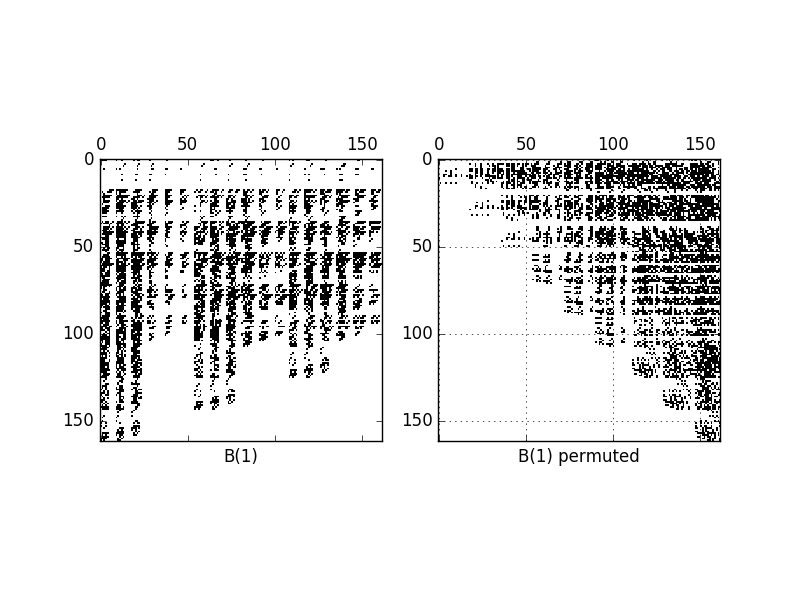
\includegraphics[width=15cm, height=8cm]{../png/sparsity.png}
\end{figure}
Dans le processus de réduction (section \ref{sec:reduction_process}), la première étape consiste à calculer le noyau de $B(1)$. Lorsque les coefficients des polynômes d'entrée sont entiers ou rationnels, ceci peut se faire de manière exacte au moyen d'un programme de calcul symbolique. La taille des entiers peut alors croître considérablement au cours des calculs et augmenter en conséquence le temps total de calcul et les besoins en mémoire du calculateur. Si par contre on veut effectuer l'ensemble des calculs en nombres flottants, ou si les coefficients d'entrée sont eux mêmes donnés sous forme numérique, alors on doit faire un calcul numérique du noyau.
La méthode éprouvée pour cela, implémentée dans des packages d'algèbre linéaire numérique comme Matlab/Octave, Numpy ou Julia, est d'effectuer une factorisation QR ``rank revealing'' de $B(1)$, que nous appellerons factorisation QRP, c'est-à-dire accompagnée de pivots sur les colonnnes. L'expérience montre que cette approche est souvent efficace mais peut s'avérer délicate à mettre en oeuvre si la taille de la matrice augmente. Montrons le sur un exemple. Nous choisissons $n =\input{../txt/n.txt}$ et un système polynomial $f$ de multidegré $\input{../txt/deg.txt}$. Seuls une quinzaine de monômes sont retenus pour chaque polynôme. Les coefficients, entiers, sont choisis aléatoirement entre $-t$ et $t$ avec, ici, $t=3$. Choisir une plus grande valeur de $t$ ne poserait aucun problème particulier si on utilise les matrices de Bezout mais on constate que le temps de calcul est excessivement long lorsqu'on utilise les bases de Grobner (voir Table \ref{tab:timings}).
Voici la liste des polynômes composant le système $f$ :\\
$f = \input{../txt/P.txt}$ \\
 La matrice de Bezout $B(1)$ est de taille $\input{../txt/Dx.txt}$ et possède une certaine structure, comme le montre la Figure \ref{fig:B1_sparsity}. Comme il parait difficile d'exploiter cette structure pour le calcul numérique du rang de la matrice $B(1)$, on doit recourir à une méthode numérique générale, par exemple une factorisation SVD ou une factorisation QRP ``rank revealing''. Choisissons cette deuxième méthode. Les termes diagonaux du facteur triangulaire $R$ seront triés en ordre décroissant, comme le montre la Figure \ref{fig:B1_diag}.
\begin{figure}[h]
  \caption{Factorisation QRP de B(1), termes diagonaux}
  \label{fig:B1_diag}
  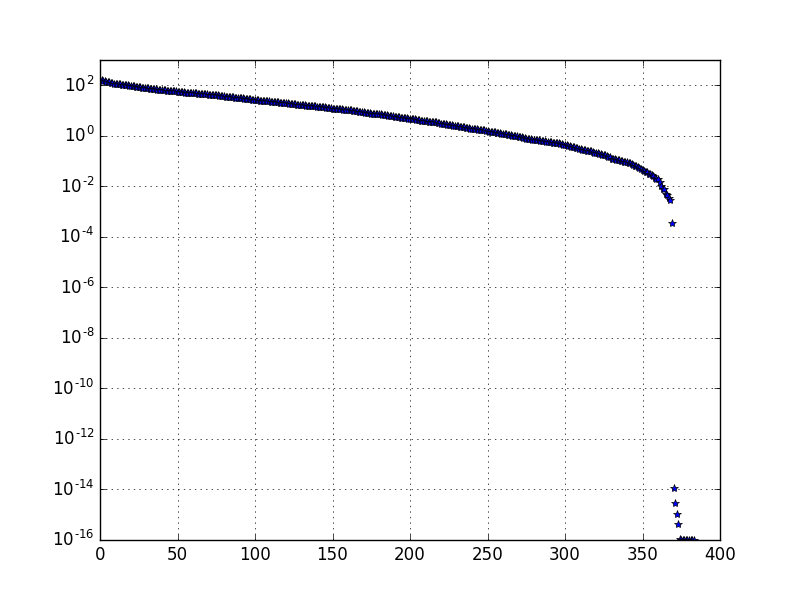
\includegraphics[width=15cm, height=8cm]{../png/bez_diag.png}
\end{figure}
On s'aperçoit que les derniers termes non nuls décroissent vite, et qu'il peut devenir difficile de choisir un seuil au dessus duquel les termes diagonaux seront déclarés ``non nuls''. Les termes non nuls s'étendent de $10^4$ à $10^{-4}$. Le saut entre termes ``non-nuls'' et termes proches du epsilon machine a tendance à diminuer à mesure que la taille de la matrice augmente, ce qui rend le calcul du rang numérique difficile.
Nous pouvons cependant améliorer, dans une certaine mesure, la situation précédente en exploitant une propriété de $B(1)$. En effet, en permutant lignes et colones de cette matrice d'une certaine façon, on peut arriver à une structure bloc-triangulaire de $B(1)$ (Figure \ref{fig:B1_diag}, subplot $2$). En appliquant à la matrice une factorisation QRP bloc après bloc, les termes diagonaux vont alors décroitre uniquement à l'intérieur de chaque bloc. La Figure \ref{fig:B1_diag}, subplot $2$, montre la nouvelle disposition des termes diagonaux à la fin de la factorisation QRP, en traitant les blocs l'un après l'autre.  Ici, les termes non nuls s'étendent de $10^0$ à $10^{-3}$. Le calcul du rang numérique est facilité et l'on trouve ici un rang égal à $\input{../txt/dim0.txt}$, qui correspond au nombre de termes dans la Figure \ref{fig:B1_diag}, subplot $2$. Enfin la Figure \ref{fig:B1_diag}, subplot $3$, montre la distribution des termes diagonaux dans la matrice finale, une fois les réductions faites, comme expliqué dans la section \ref{sec:reduction_process}. On voit que la distribution des termes est très proche de celle précédent les réductions. Le rang de la nouvelle matrice est $\input{../txt/dim.txt}$, c'est la dimension du quotient $A$, d'après la proposition~\ref{conjecture}.


\end{document}
